\documentclass[12pt]{article}
\usepackage[english, polish]{babel}
\usepackage{polski}
\usepackage[utf8]{inputenc}
\usepackage{mathtools}
\usepackage{amsfonts}
\usepackage{amsmath}
\usepackage{amsthm}

\usepackage{booktabs}
\usepackage{csquotes}
% Ponieważ `csquotes` nie posiada polskiego stylu, można skorzystać z mocno zbliżonego stylu chorwackiego.
\DeclareQuoteAlias{croatian}{polish}

% Użyj czcionki kroju Courier.
\usepackage{courier}


\usepackage{listings}
\lstloadlanguages{TeX}

\lstset{
	literate={ą}{{\k{a}}}1
           {ć}{{\'c}}1
           {ę}{{\k{e}}}1
           {ó}{{\'o}}1
           {ń}{{\'n}}1
           {ł}{{\l{}}}1
           {ś}{{\'s}}1
           {ź}{{\'z}}1
           {ż}{{\.z}}1
           {Ą}{{\k{A}}}1
           {Ć}{{\'C}}1
           {Ę}{{\k{E}}}1
           {Ó}{{\'O}}1
           {Ń}{{\'N}}1
           {Ł}{{\L{}}}1
           {Ś}{{\'S}}1
           {Ź}{{\'Z}}1
           {Ż}{{\.Z}}1,
	basicstyle=\footnotesize\ttfamily,
}

% ------------------------

\AtBeginDocument{
	\renewcommand{\tablename}{Tabela}
	\renewcommand{\figurename}{Rys.}
}

% ------------------------
% --- < tabele > ---

\usepackage{array}
\usepackage{tabularx}
\usepackage{multirow}
\usepackage{booktabs}
\usepackage{makecell}
\usepackage[flushleft]{threeparttable}
\usepackage{graphicx}
\usepackage{wrapfig}

\newcommand{\HRule}[1]{\rule{\linewidth}{#1}} 	% Horizontal rule

\makeatletter							% Title
\def\printtitle{%						
    {\centering \@title\par}}
\makeatother									

\makeatletter							% Author
\def\printauthor{%					
    {\centering \large \@author}}				
\makeatother							

% --------------------------------------------------------------------
% Metadata (Change this)
% --------------------------------------------------------------------
\title{	\normalsize \textsc{Big data} 	% Subtitle
		 	\\[2.0cm]								% 2cm spacing
			\HRule{0.5pt} \\						% Upper rule
			\LARGE \textbf{\uppercase{Problem klasyfikacji - cukrzyca}}	% Title
			\HRule{2pt} \\ [0.5cm]		% Lower rule + 0.5cm spacing
			\normalsize \today			% Todays date
		}

\author{
		Emilia Lubos\\
		Daria Pacewicz\\
		Michał Gandor\\		
}
\begin{document}
% ------------------------------------------------------------------------------
% Maketitle
% ------------------------------------------------------------------------------
\thispagestyle{empty}		% Remove page numbering on this page

\printtitle					% Print the title data as defined above
  	\vfill
\printauthor				% Print the author data as defined above

\newpage
\tableofcontents
\newpage
\section{Opis zbioru danych}

Zbiór zawiera informacje czy u danego pacjenta występuje cukrzyca czy też nie. Pacjentami są kobiety w wieku 21 lat lub starszych pochodzących z Indii. Opis dokonany jest za pomocą zmiennych:

\begin{itemize}
\item Pregnancies - ilość ciąż,
\item Glucose - koncentracja glukozy wg 2-godzinnego testu,
\item BloodPressure - rozkurczowe ciśnienie krwi (mm Hg),
\item SkinThickness - grubość fałdu skóry na tricepsie (mm),
\item Insulin - poziom insuliny mierzony (mu U/ml)
\item BMI - index BMI (waga w kg/(wzrost w $m^2$)
\item DiabetesPedigreeFunction - funkcja rodowodu cukrzycy,
\item Age - wiek w latach,
\item Outcome - 0 = wynik negatywny (brak cukrzycy), 1 = wynik pozytywny (cukrzyca).
\end{itemize}

Rozkład klas:

\begin{itemize}
\item 0 - 500 próbek
\item 1 - 268 próbek
\end{itemize}

\begin{figure}
	\centering
	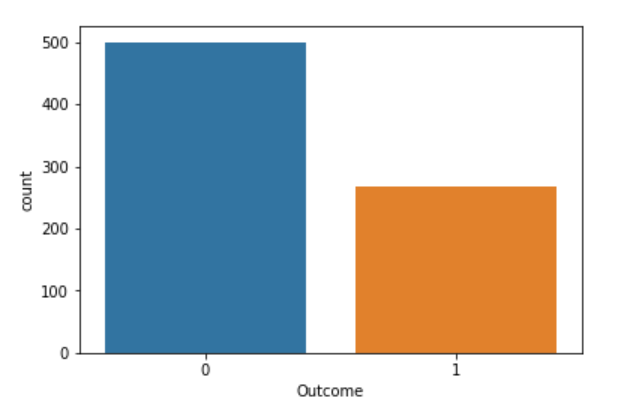
\includegraphics{images/outcome.png}
	\caption{Outcome}
	\label{fig:outcome}
\end{figure}

Całkowita liczba obserwacji wynosi 786.

Źródło: https://www.kaggle.com/uciml/pima-indians-diabetes-database


\pagebreak
\section{Cel projektu}

Celem projektu jest dokonanie klasyfikacji oraz zbadanie czy u danego pacjenta wystąpi cukrzyca czy nie. Zbadane zostanie także czy dane zawarte w~zbiorze są wystarczające do decyzji o prawdopodobieństwie wystąpienia choroby oraz czy wszystkie z nich wpływają znacząco na wystąpienie choroby.
W projekcie porównane zostaną wyniki skuteczności różnych klasyfikatorów.

\section{Narzędzia}
	W tym projekcie posłużono się językiem Python oraz bibliotekom poświęconym analizie danych i uczeniu maszynowym, takimi jak: NumPy, Pandas, SciKit-learn. Do wytworzenia wykresów zastosowano biblioteki Matplotlib oraz Seaborn.


\section{Analiza zbioru}

Zanim przystąpimy do próby klasyfikacji dane muszą zostać odpowiednio przygotowane. Sprawdzone zostają wiersze w których występują zera oraz wartości odstające.

\subsection{Wartości zerowe}

\begin{figure}
	\centering
	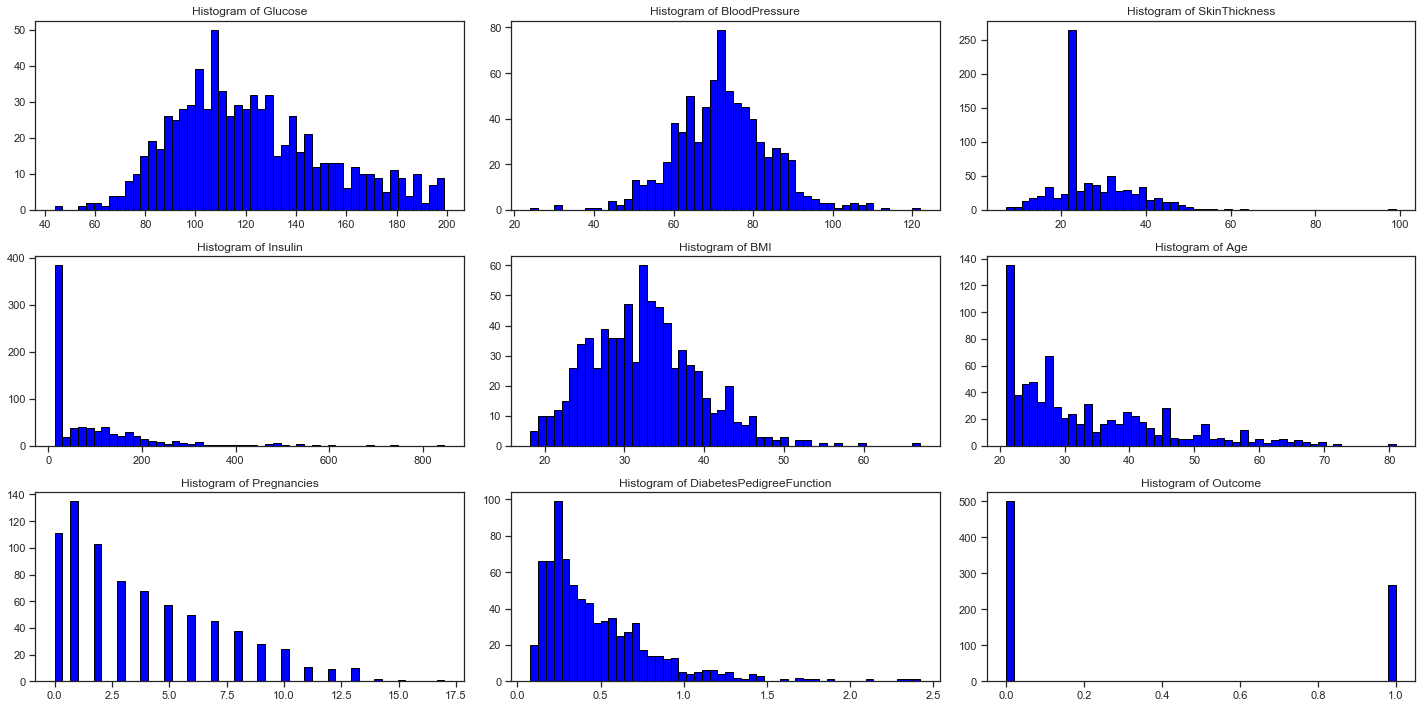
\includegraphics[width=1.2\textwidth]{images/hist_median.png}
	\caption{Histogramy po zastąpieniu wartości 0 medianą}
	\label{fig:outliers}
\end{figure}

\begin{figure}
	\centering
	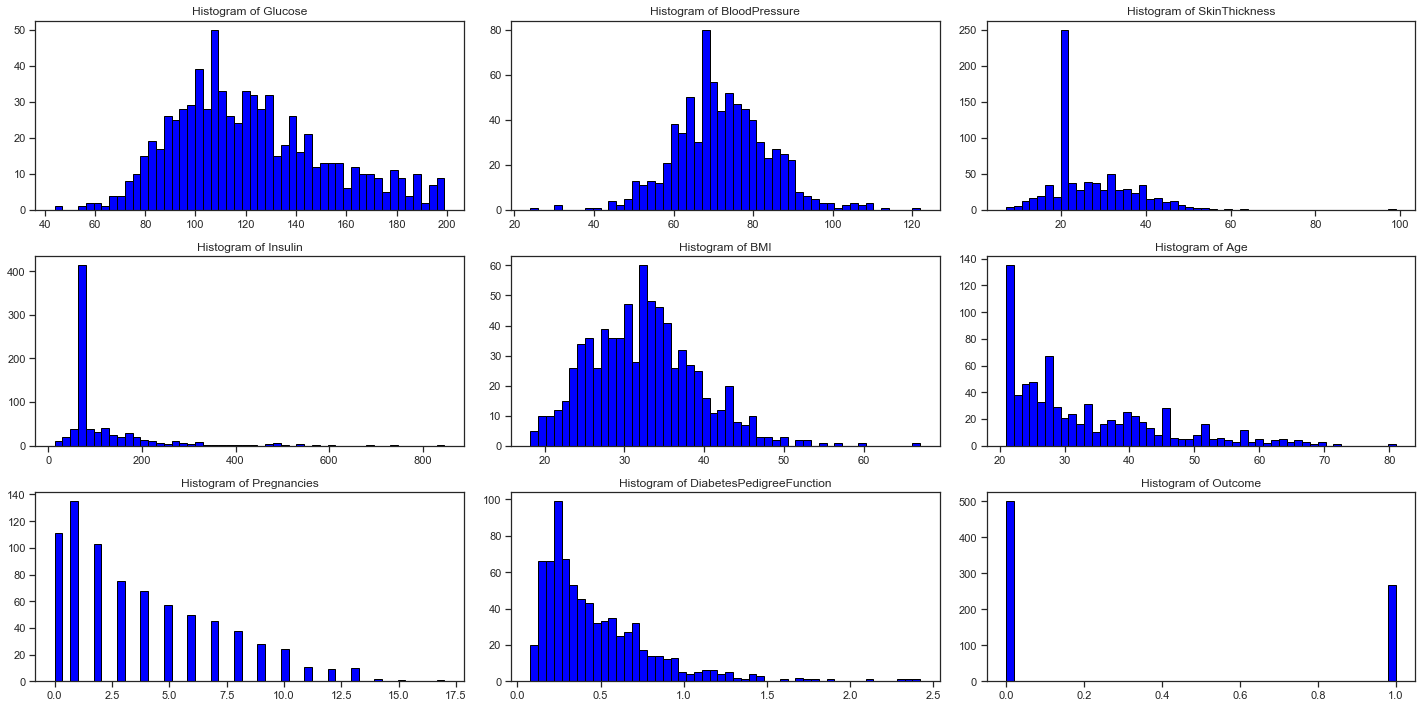
\includegraphics[width=1.2\textwidth]{images/hist_average.png}
	\caption{Histogramy po zastąpieniu wartości 0 średnią}
	\label{fig:outliers}
\end{figure}

Z tabel wynika, że istnieją wartości zerowe w kolumnach \textit{Pregnancies, Glucose, BoloodPressuure, SkinThickness, Insulin, BMI}. Z medycznego punktu widzenia cechy w badanym zbiorze nie mogą być równe zeru, świadczy to o braku poprawności danych danych. W~przypadku pierwszej kolumny wartości zerowe są poprawne - jest to informacja, że dana kobieta nie była w~ciąży. W przypadku reszty obserwacji dane zostają zamienione na \textbf{średnią wartość} w kolumnie, \textbf{medianę} oraz zostają całkowicie \textbf{usunięte}. Oba trzy przypadki posłużą jako dane testowe.

% Please add the following required packages to your document preamble:
\begin{table}[]
\begin{tabular}{@{}llllllllll@{}}
\toprule
               & \textbf{Pregnancies} & \textbf{Glucose} & \textbf{BloodPressure} & \textbf{SkinThickness} & \textbf{Insulin} &  &  &  &  \\ \midrule
\textbf{count} & 768                  & 768              & 768                    & 768                    & 768              &  &  &  &  \\
\textbf{mean}  & 3.845052             & 120.8945         & 69.10547               & 20.53646               & 79.79948         &  &  &  &  \\
\textbf{std}   & 3.369578             & 31.97262         & 19.35581               & 15.95222               & 115.244          &  &  &  &  \\
\textbf{min}   & 0                    & 0                & 0                      & 0                      & 0                &  &  &  &  \\
\textbf{25\%}  & 1                    & 99               & 62                     & 0                      & 0                &  &  &  &  \\
\textbf{50\%}  & 3                    & 117              & 72                     & 23                     & 30.5             &  &  &  &  \\
\textbf{75\%}  & 6                    & 140.25           & 80                     & 32                     & 127.25           &  &  &  &  \\
\textbf{max}   & 17                   & 199              & 122                    & 99                     & 846              &  &  &  &  \\ \bottomrule
\end{tabular}
\end{table}

% Please add the following required packages to your document preamble:
\begin{table}[]
\begin{tabular}{@{}llllllllll@{}}
\toprule
               & \textbf{BMI} & \textbf{DiabetesPedigreeFunction} & \textbf{Age} & \textbf{Outcome} & \textbf{} &  &  &  &  \\ \midrule
\textbf{count} & 768          & 768                               & 768          & 768              &           &  &  &  &  \\
\textbf{mean}  & 31.99258     & 0.471876                          & 33.24089     & 0.348958         &           &  &  &  &  \\
\textbf{std}   & 7.88416      & 0.331329                          & 11.76023     & 0.476951         &           &  &  &  &  \\
\textbf{min}   & 0            & 0.078                             & 21           & 0                &           &  &  &  &  \\
\textbf{25\%}  & 27.3         & 0.24375                           & 24           & 0                &           &  &  &  &  \\
\textbf{50\%}  & 32           & 0.3725                            & 29           & 0                &           &  &  &  &  \\
\textbf{75\%}  & 36.6         & 0.62625                           & 41           & 1                &           &  &  &  &  \\
\textbf{max}   & 67.1         & 2.42                              & 81           & 1                &           &  &  &  &  \\ \bottomrule
\end{tabular}
\end{table}

\subsection{Wartości odstające}

\begin{figure}
	\centering
	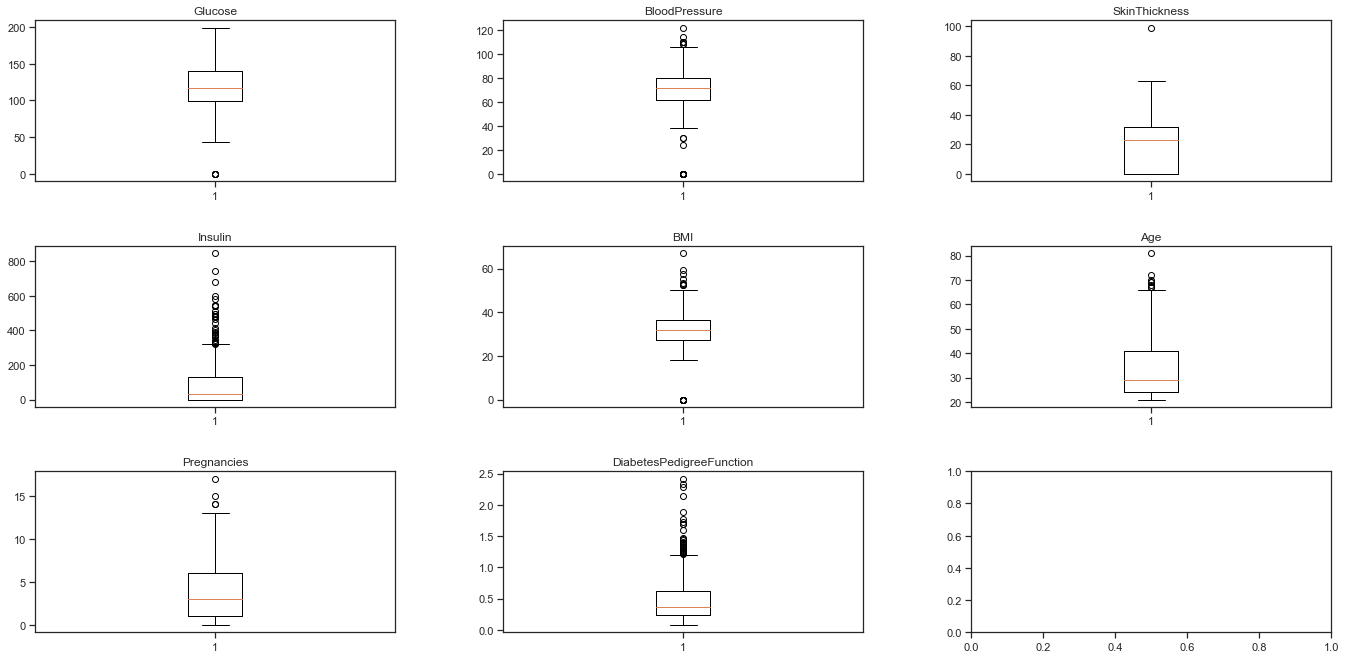
\includegraphics[width=1.2\textwidth]{images/outliers.png}
	\caption{Wartości odstające}
	\label{fig:outliers}
\end{figure}

\begin{itemize}
\item Pregnancies

	Brak wartości odstających.
\item Glucose 

	Według badań medycznych poziom cukru poniżej 140mg/dl jest wynikiem prawidłowym. Ponad 200mg/dl świadczy o wystąpieniu cukrzycy \cite{sugarLevel}.
\item BloodPressure 

	Rozkurczowe ciśnienie tętnicze uznawane jest za poprawne w granicach 60-80 mm/Hg. Poniżej tego progu zostaje stwierdzona chorba. Ciśnienie nie może być mniejsze niż 40 \cite{pressure}.
\item SkinThickness


\item Insulin - poziom insuliny mierzony (mu U/ml)
\item BMI 

	Zakres BMI waha się pomiędzy 16 a 40. Gdzie 16 to wygłodzenie, a wartości powyżej 40 to 3 stopień otyłości \cite{bmi}. Wiersz wykraczające poza ten zakres powinny zostać usunięte ze zbioru.
	
\item DiabetesPedigreeFunction - funkcja rodowodu cukrzycy,
\item Age
	
	Brak wartości odstających.

\end{itemize}
\subsection{Selekcja cech}
	Z modelu zostały usunięte cechy które nie zostały uznane za istotne. Kolumny które pozostaną w modelu zostały wybrane z użyciem ExtraTreesClassifier. Cechy z najniższym wynikiem zostają odrzucone.  
\subsection{Normalizacja}
	Dane zostały znormalizowane. Wszystkie wartości są teraz z zakresu 0-1. Do normalizacji użyto MinMaxScaler i StandardScaler.

\section{Walidacja krzyżowa}
	Przed przystąpieniem do klasyfikacji zastosowano prosty podział zbioru danych na dane treningowe oraz testowe oraz 5-krotną walidację krzyżową. Zdecydowano się na podział zbioru w następującej proporcji: 70\% - dane treningowe, 30\% - dane testowe. Podział ten zastosowano do wyboru najlepszych parametrów modeli klasyfikacji. 
	Walidację krzyżową stosuje się w celu minimalizacji problemu nadmiernego dopasowania (\textit{overfitting}). Dzięki niej można uzyskać informacje takie jak dokładność modelu (accuracy) czy macierz pomyłek, które umożliwiają ocenę jakości modelu.
	
\section{Klasyfikacja}
	Do klasyfikacji zostało użytych sześć różnych klasyfikatorów w celu porównania wyników.

Tu można dodać coś o wybranych parametrach i dlaczego takie....

\begin{itemize}
\item{Maszyna wektorów nośnych (SVN)}
\item{K najbliżych sąsiadów (KNN)}
\item{Drzewo decyzyjne}
\item{Las losowy}
\item{Regresja logistyczna}
\item{Naiwny klasyfikator bayesowski}

\end{itemize}

\section{Wyniki}


\begin{thebibliography}{9}

\bibitem{sugarLevel}
	https://www.diabetes.co.uk/diabetescare/blood-sugar-level-ranges.html
\bibitem{pressure}
	http://www.bloodpressureuk.org/BloodPressureandyou/Thebasics/Bloodpressurechart)

\bibitem{bmi}
	https://pl.wikipedia.org/wiki/Wskaźnikmasyciała
\end{thebibliography}


\end{document}